%!TEX root = ../09-Photoelectric-Effect.tex
\chapter{Properties of High-Impedance Buffer Amplifier}
\begin{figure}
	\centering
	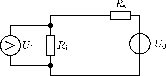
\includegraphics[width=0.5\textwidth]{./img/2-1-sch.pdf}
	\caption{Schematic for determining the electrometer's input impedance}
	\label{fig:elec_in_im}
\end{figure}

\section{Ideal Current and Voltage Sources}
An ideal current source is an electronic circuit that delivers an electric current, independent of the voltage across it.
Thus, it must have an infinite impedance.
An ideal voltage source, on the other hand, maintains a constant voltage across its terminals, independent of its load or output current.
Therefore, it has to have a vanishing resistance.

\section{Am- and Voltmeters}
An ideal ammeter is a device used for measuring an electric current of a circuit.
Most modern ammeters use the voltage drop over a precision resistor, called a shunt, with known resistance.
The flowing current can be calculated by using \texttt{Ohm}'s law.
Classical ammeters are connected in series with the circuit carrying the current, so their shunts need to have a very low impedance to cause little additional voltage drop, which could affect the circuit.
A voltmeter is an instrument used for measuring a potential difference, a voltage, between two points in an electric circuit.
Usually, it is connected in parallel with the part of the circuit whose voltage has to be measured, so its impedance should be infinitely high to not present an additional load to the circuit.

\section{Photoelectric Cells}
A photoelectric cell is a gas-filled or vacuum tube containing a so called photocathode and -anode.
Incoming photons knock out electrons out of the cathode's surface by the photoelectric effect, some of which are collected by the anode.%not neccessarily attracted
The cell's current thus is dependent on the frequency and intensity of the incoming photons, whereas its spectral response is dependent on the cathode's material, since different materials have different workfunctions.

\section{Determination of the Input Impedance}
\begin{table}[b!]
	\centering
	\caption[Series resistance over amplifier voltage]{Series resistance over amplifier voltage, $U_0=\SI{5}{\volt}$ at $\nu=1$}
	\label{tab:impedance}
	\begin{tabular}{cS}
		\toprule
		{resistance in \si{\ohm}}	&	{amplifier voltage in \si{\volt}}	\\
		\midrule
			$10^8$	&	4.999	\\
			$10^9$	&	4.988	\\
			$10^{10}$	&	4.9	\\
		\midrule
		{mean input impedance}	&	\SI{4.69(38)e11}{\ohm}\\
		\bottomrule
	\end{tabular}
\end{table}
To measure the input impedance of an electrometer, consisting of a high-impedance buffer amplifier, the circuit in \autoref{fig:elec_in_im} is built.
A fixed voltage of \SI{5}{\volt} is applied, varying the series resistor and measuring the voltage drop across the amplifier's terminals.

Using \texttt{Kirchhoff}'s first and second rule, it holds that
\begin{align}
	U_1	&= 	R_\text{i}\cdot I \label{eq:kirch_1}\qquad(\nu = 1)\\
	I 					&=	\frac{U_0}{R_\text{s}+R_\text{i}},	\label{eq:kirch_2}
\end{align}
where $\nu$ denotes amplification.

Rearranging equations \ref{eq:kirch_1} and \ref{eq:kirch_2} yields
\begin{equation}
	R_\text{i}=R_\text{s}\cdot\frac{U_1}{U_0-U_1},
\end{equation}
which can be used to compute the input impedance.

\autoref{tab:impedance} shows the measured values for the specified setup.
The amplifier's input impedance is calculated as a mean value of \SI{4.69(38)e11}{\ohm}, which matches the manufacturer's specification of $R_\text{i}\leq\SI{e13}{\ohm}$.
